\subsection{Project Summary}
\begin{frame}
\frametitle{Sprint One}
\textbf{Main purpose:}\\
\centering
\only<1>{Bug fixing\\ \includegraphics[height=4cm]{images/bugfixing}}
\only<2>{Improve Drawer\\ 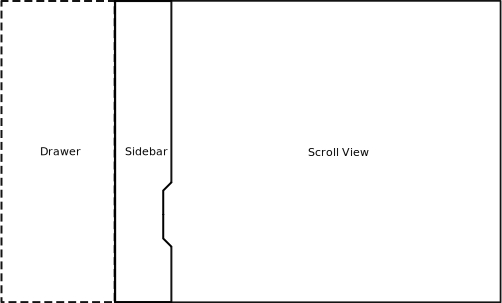
\includegraphics[height=4cm]{images/drawer}}
\only<3>{Carry out functional tests\\\includegraphics[height=4cm]{images/test}}
\end{frame}

\begin{frame}
\frametitle{Sprint One}
\begin{center}
Intermediate Product Demonstration
\end{center}

\end{frame}

\begin{frame}
\frametitle{Sprint Two}
\textbf{Main purpose:}\\
\centering
\only<1>{Create Prototypes of Settings \quad\includegraphics[height=4cm]{images/prototype}}
\only<2>{Receive feedback from customer meetings \quad\includegraphics[height=4cm]{images/customer}}

\end{frame}

\begin{frame}
\frametitle{Sprint Three}
\textbf{Main purpose:}
\textbf{Start implementation of Settings:}\\
\begin{columns}
\begin{column}{0.5\textwidth}

          \begin{center}
\only<2,3,4,5>{Settings for Launcher\\
           	 \includegraphics[height=2cm]{images/giraf}}
        \end{center}
        \begin{center}
       		\only<3,4,5>{Application Management\\
             \includegraphics[height=2cm]{images/apps}}
        \end{center}
\end{column}
\begin{column}{0.5\textwidth}
        \begin{center}
               		\only<4,5>{Cars\\
                     \includegraphics[height=2cm]{images/cars}}
         \end{center}
        \begin{center}
                    \only<5> {Sequence\\
                     \includegraphics[height=2cm]{images/sequence}}
        \end{center}
\end{column}
\end{columns}
\end{frame}

\begin{frame}
\frametitle{Sprint Four}
\textbf{Main purpose:}\\
\begin{center}
IDA testing\\
\only<1>{\includegraphics[height=3cm]{images/usertest}\\}
\pause
{ Finish implementation of Settings}\\
\end{center}
\end{frame}

\begin{frame}
\frametitle{Sprint Four}
\begin{center}
Final Product Demonstration
\end{center}
\end{frame}